\documentclass{../llncs2e/llncs}
\usepackage{inputenc}
\usepackage{graphicx}
\usepackage{caption}
% page numbering
\pagestyle{plain}
% change the spacing between the caption and the table
\captionsetup[table]{skip=10pt}
% -------------------------------------------------------------------------------------------------
% CLOUD4THINGS: automatic provisioning of smart places infrastructure
% -------------------------------------------------------------------------------------------------
\title{Cloud4Things: automatic provisioning of smart places infrastructure}
% -------------------------------------------------------------------------------------------------
% AUTHORS
% -------------------------------------------------------------------------------------------------
 \author{\Large Marcus Gomes, Miguel Pardal}
% -------------------------------------------------------------------------------------------------
% INSTITUTION
% -------------------------------------------------------------------------------------------------∫
 \institute{\large T\'ecnico Lisboa, Universidade T\'ecnica de Lisboa\\
 \email{\{marcus.paulino.gomes, miguel.pardal\}@tecnico.ulisboa.pt}}
% -------------------------------------------------------------------------------------------------
% DOCUMENT
% -------------------------------------------------------------------------------------------------
\begin{document}
\maketitle
% -------------------------------------------------------------------------------------------------
% ABSTRACT
% -------------------------------------------------------------------------------------------------
\begin{abstract}
Smart places are an ecosystem composed by sensors - e.g. RFID tags - actuators - e.g. automatic doors -
and computing infrastructure - e.g. cloud servers - that are able to acquire data about the surrounding
environment and use that data to improve the experience of the people using the place.The data acquired
by the sensors needs to be collected, interpreted and transformed into information that is used to gather
knowledge about the smart place. A complete example of a platform that allows the transformation of sensor
data into information is Fosstrak, an open source RFID software that implements the EPC Network standards.
In this paper we propose Cloud4Things, a solution that automates the provisioning of RFID software in the
cloud by relying on configuration management tools that leverage existing stacks. We will perform a qualitative
evaluation of our solution based on Docker containers with other solutions, such as full Virtual Machines,
or tools implementing the TOSCA standards. The current prototype is able to support stages in the lifecycle of
a smart place, from initial provisioning and day-to-day operation.
\end{abstract}
% -------------------------------------------------------------------------------------------------
% INTRODUCTION
% -------------------------------------------------------------------------------------------------
\section{Introduction}
\label{sec:introduction}
In this section we will describe the problem that we want to solve with Cloud4Things, i.e, automating
the configuration and provisioning of smart places applications based on the RFID technology in the
Cloud, in our case the Fosstrak platform, that implements the GS1 EPC Network specifications.

Cloud4Things will perform the automatic provisioning aiming the required software stack by the smart
place infrastructure and the application performance.

We also will give some examples of smart places and describe the life-cycle of a smart place
application and point out what are the stages that will be the target of our work.
% -------------------------------------------------------------------------------------------------
% RELATED WORK
% -------------------------------------------------------------------------------------------------
\section{Related Work}
\label{sec:related_work}
In this section we will describe the most relevant work that is related with Cloud4Things, starting
by the work developed by Guinard and Floerkmeier (EPC Cloud), and later by presenting the other
solutions related with our work such as TOSCA, automatic provisioning with configuration management
tools + VMs and proprietary solutions such as Amazon VM import and Amazon Elastic Beanstalk.

% ----------------------------------------
% INTERNET OF THINGS AND CLOUD COMPUTING
% ----------------------------------------
\subsubsection{EPC Cloud}
\label{subs:epc-cloud}
In RFID-based IoT applications, Guinard et al. \cite{guinard2011cloud} point out that the
deployment of RFID applications are cost-intensive mostly because they involve the
deployment of often rather large and heterogeneous distributed systems. As a consequence,
these systems are often only suitable for big corporations and large implementations and
do not fit the limited resources of small to mid-size businesses and small scale applications
both in terms of required skill-set and costs. To address this problem, Guinard et al. propose
a Cloud-based solution that integrates virtualization technologies and the architecture of
the Web and its services. The case of study consists in a IoT application that uses RFID technology
to substitute existing Electronic Article Surveillance (EAS) technology, such as those used in
clothing stores to track the products. In this scenario they applied the Utility Computing blueprint
to the software stack required by the application using the AWS platform and the EC2 service. To
evaluate the Cloud-based solution, two prototypes was successfully implemented to prove that
the pain points of the RFID applications can be relaxed by adopting the proposed solution.\\

% ---------------------------------------------
% TOSCA
% ---------------------------------------------
\subsubsection{TOSCA}
\label{subs:tosca}
TOSCA (Topology and Orchestration Specification for Cloud Applications) \cite{li2013towards} is
proposed in order to improve the reusability of service management processes and automate IoT application
ratified by OASIS in \cite{} deployment in heterogeneous environments. TOSCA is a new cloud standard to formally
describe the internal topology of application components and the deployment process of Cloud applications.
The structure and management of IT services is specified by a meta-model, which consists of
a \textit{Topology Template}, that is responsible for describing the structure of a service, then there
are the \textit{Artifacts}, that describe the files, scripts and software components necessary to be
deployed in order to run the application, and finally the \textit{Plans}, that defined the management process
of creating, deploying and terminating a service. The correct topology and management procedure can be inferred
by a TOSCA environment just by interpreting the topology template, this is known as ``declarative" approach.
Plans realize an ``imperative" approach that explicitly specifies how each management process should be done.
The topology templates, plans and artifacts of an application are packaged in a Cloud Service Archive (.csar file)
and deployed in a TOSCA environment, which is able to interpret the models and perform the specified management
operations. These .csar files are portable across different Cloud providers, which is a great benefit in terms
of deployment flexibility. To evaluate its feasibility, TOSCA was used in the specification of a typical
application in building automation. an application to control an Air Handling Unit (AHU). The common IoT
components, such as gateways and drivers will be modeled, and the gateway-specific artifacts that are
necessary for application deployment will also be specified. By archiving the previous specifications
and corresponding artifacts into a .csar file, and deploying it in a TOSCA environment, the deployment
of AHU application onto various gateways can be automated. As a newly established standard to counter
growing complexity and isolation in cloud applications environments, TOSCA is gaining momentum in industrial
adoption as well for academic interest.\\

% -------------------------------------------------------------------------------------------------
% SOLUTION ARCHITECTURE
% -------------------------------------------------------------------------------------------------
\section{Solution}
\label{sec:solution}
In this section we will describe the solution of work, i.e, Cloud4Things architecture:
% -------------------------------------------------------------------------------------------------
% DOCKER
% -------------------------------------------------------------------------------------------------
\subsection{Docker}
\label{sub:docker}
In this section we will introduce Docker and explain what are the advantages offered by this
platform that will contribute to make our solution more efficient. We also will present a detailed
explanation about the architecture of the Fosstrak stack and how it is Dockerized.

- Explain what is the DOcker containers and its advantages
- Show the figure that shows how the stack is organized (Demo figure)
% -------------------------------------------------------------------------------------------------
% AUTOMATIC PROVISIONING
% -------------------------------------------------------------------------------------------------
\subsection{Automatic Provisioning}
\label{sub:Automatic Provisioning}
In this section we will introduce the configuration management tools, in particular Chef, and then
we will present a detailed explanation about how we use Chef to perform the automatic provisioning
in the Cloud providers, in our case AWS, but by using Chef it is possible to port the
infrastructure to others providers.
\begin{figure}
  \centering
  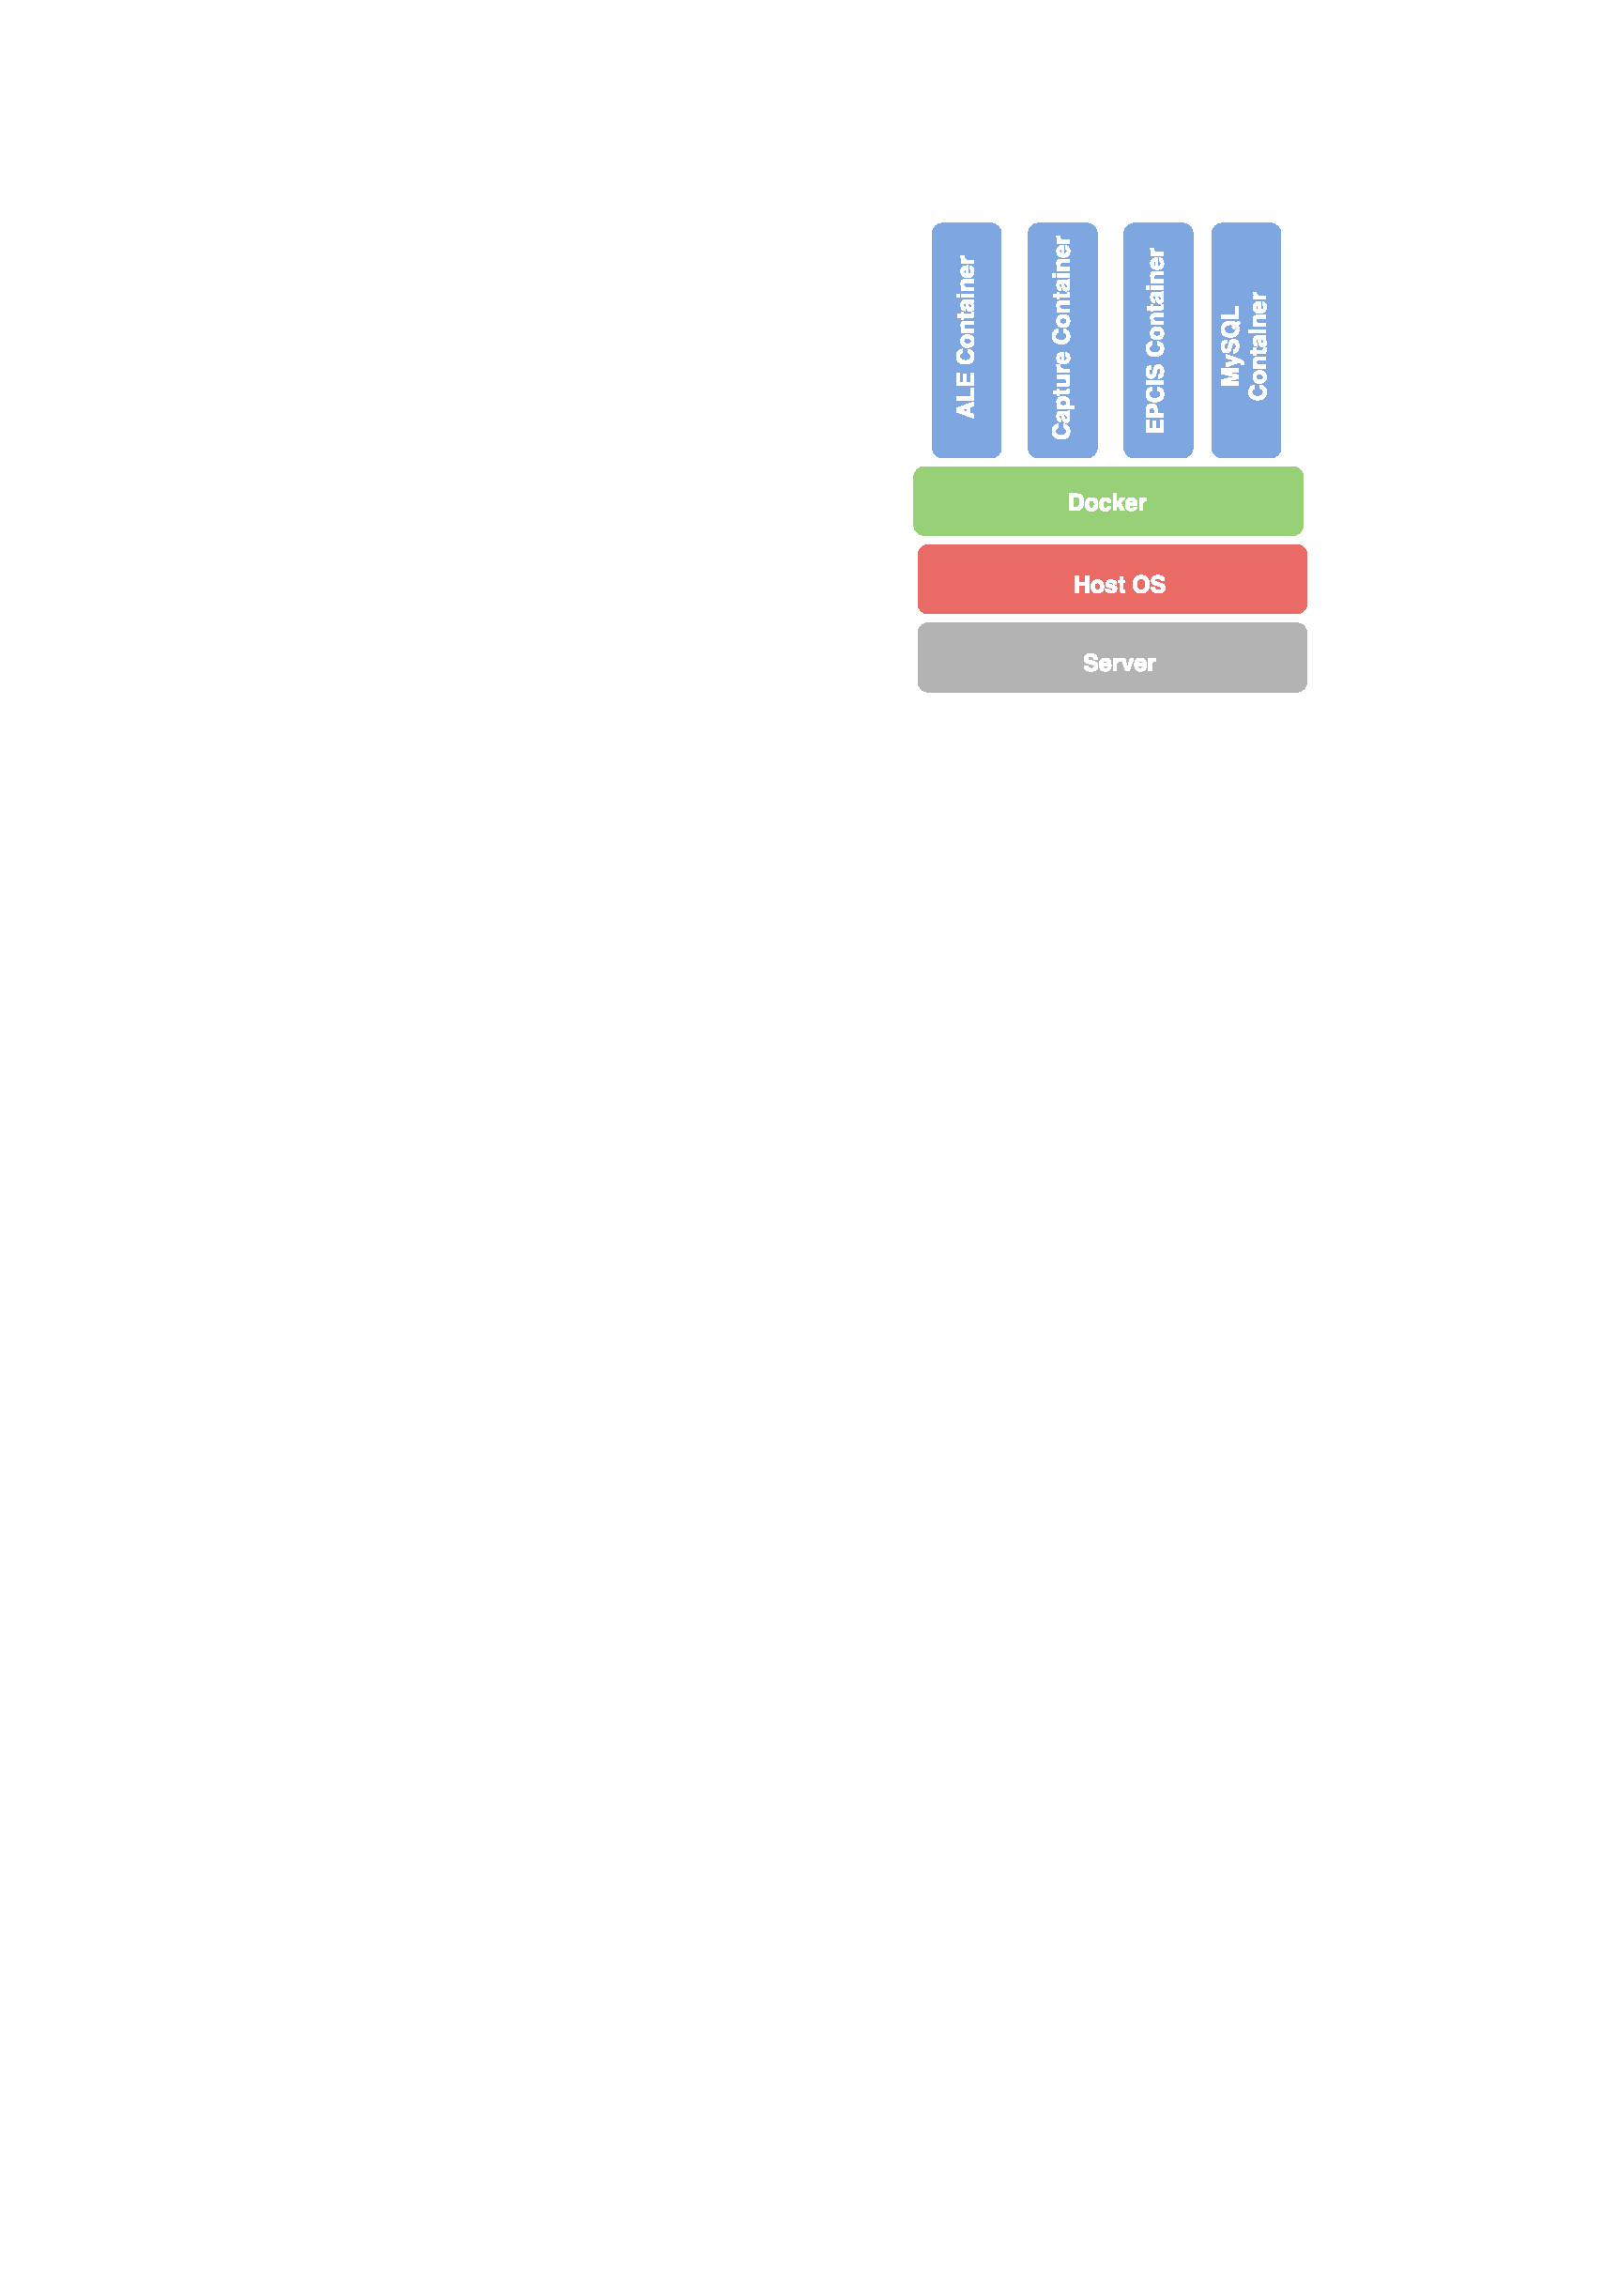
\includegraphics[width=.5\textwidth]{images/docker-stack}
\end{figure}
% -------------------------------------------------------------------------------------------------
% SMART PLACE AUTOMATIC CONFIGURATION
% -------------------------------------------------------------------------------------------------
\subsection{Smart Place Automatic Configuration}
\label{sub:Smart Place Automatic Configuration}
In this section we will introduce the Cloud4Things CLI, a command line interface that allows the
users to upload a predefined configuration of a smart place to the Fosstrak server. We will explain
the procedures required to configure a smart place, i.e, the template that is used to describe the
configuration.
% -------------------------------------------------------------------------------------------------
% QUALITATIVE EVALUATION
% -------------------------------------------------------------------------------------------------
\section{Qualitative Evaluation}
\label{sec:qualitative_evaluation}
In this section we will perform a qualitative evaluation of the developed work until the date. The
evaluation consists in compare the efficiency of the software stack required by our solution with
the other alternative solutions that are mentioned in the Related Work.

Another component that can be evaluated is the process to configure a smart place based on the
Fosstrak platform. In the standard solution there are two implemented clients that can be used to
configure the readers and events that belongs to a smart place. However, configure a smart place
with those clients is a manual process that is ineffective and error prone. In order to turn this
configuration process more automatic, our approach is to provide a client application that allows
the user to describe the smart place configuration in a JSON file, that later will be used by the
client to setup the readers and events in the application that is running in the Cloud.
% -------------------------------------------------------------------------------------------------
% CONCLUSION
% -------------------------------------------------------------------------------------------------
\section{Conclusion}
\label{sec:conclusion}
In this section we will present the conclusion of the paper and also we will discuss about some
enhancements of our work.

At the top of the Future Work list is the measure of the elasticity of the application regarding
the events that occur in the physical world. Currently our solution is centralized, i.e, all the
container that runs the Fosstrak application are located in the same machine, a important component
of our work is to compare the current approach with a distributed solution. Finally, the client
application still is textual, in the future a important feature that can be added to our solution
is a GUI that allows the user to have a more visual perspective of the configuration of the smart
place.
% -------------------------------------------------------------------------------------------------
% BIBLIOGRAPHY
% -------------------------------------------------------------------------------------------------
%\bibliographystyle{ieeetr}
%\bibliography{}
\end{document}
